% ============================================================
% 上证综指波动率建模与预测
% 基于 ARIMA-GARCH 族模型的实证分析
% 编译: xelatex analysis_report.tex
% ============================================================

\documentclass[12pt,a4paper]{ctexart}

% ---- 页面设置 ----
\usepackage[top=2.5cm, bottom=2.5cm, left=3cm, right=3cm]{geometry}
\usepackage{setspace}
\onehalfspacing

% ---- 数学与符号 ----
\usepackage{amsmath,amssymb,amsfonts}
\usepackage{bm}

% ---- 图表与浮动体 ----
\usepackage{graphicx}
\usepackage{float}
\usepackage{booktabs}
\usepackage{multirow}
\usepackage{array}
\usepackage{caption}
\captionsetup[table]{font={small},skip=4pt}
\captionsetup[figure]{font={small},skip=4pt}

% ---- 超链接与引用 ----
\usepackage[colorlinks=true,
            linkcolor=black,
            citecolor=black,
            urlcolor=blue]{hyperref}

% ---- 自定义命令 ----
\newcommand{\E}{\mathbb{E}}
\newcommand{\condvar}{\sigma_t^2}

\begin{document}

% ========== 标题页 ==========
\begin{center}
\vspace{2cm}
{\LARGE \textbf{上证综指波动率建模与预测}}\\[8pt]
{\large \textbf{——基于ARIMA-GARCH族模型的实证分析}}\\[1.5cm]
{\large 时间序列分析课程报告}\\[1cm]
{\large \today}
\end{center}

\vspace{2cm}
\begin{center}
\rule{0.8\linewidth}{0.4pt}
\end{center}

\newpage

% ========== 摘要 ==========
\begin{abstract}
\noindent
股票市场波动率的精准度量与预测是金融风险管理、资产定价及政策制定的核心议题。中国A股市场因其独特的制度环境与投资者结构，收益率呈现出显著的“尖峰厚尾”、波动率聚集及非对称性等复杂特征，对传统建模方法提出了挑战。本文以2000年1月至2026年6月上证综指的日度数据为样本，系统构建并比较了ARIMA-GARCH(1,1)-Normal、ARIMA-GARCH(1,1)-$t$、ARIMA-EGARCH(1,1)-$t$及ARIMA-APARCH(1,1)-$t$四种模型在波动率拟合与预测中的表现。研究遵循“均值方程过滤—条件异方差检验—波动率建模—滚动预测评估”的规范流程。结果表明：在样本内拟合方面，引入学生$t$分布与杠杆效应的EGARCH(1,1)-$t$模型表现最优（AIC=20379.58），其自由度参数（$\nu=4.77$）与杠杆项系数均高度显著，有力验证了收益率的厚尾性与波动率的非对称响应；在样本外滚动预测方面，EGARCH(1,1)-$t$模型同样以最低的RMSE（0.8181）和MAE（0.5975）保持领先，而APARCH(1,1)-$t$模型则在QLIKE损失函数下表现最佳（0.9289）。Diebold-Mariano检验进一步确认了非对称模型相对对称模型的预测优势具有统计显著性。本文研究不仅为上证综指波动率刻画提供了稳健的模型选择参考，更揭示了在金融建模中合理平衡模型复杂度与泛化能力的重要性。

\vspace{8pt}
\noindent\textbf{关键词：}上证综指；GARCH模型；EGARCH模型；APARCH模型；波动率预测；滚动窗口

\end{abstract}

\newpage
\tableofcontents
\newpage

% ========== 1. 引言 ==========
\section{引言}

股票市场波动率作为资产价格不确定性的量化表征，是现代金融学风险管理、资产定价及货币政策制定的核心输入变量。有效的波动率度量与预测，不仅关乎金融机构的资产配置与风险预算，也是监管当局实施逆周期调节与压力测试的重要依据。作为中国资本市场的旗舰指数，上证综指的历史走势深刻烙印着宏观经济变迁与市场制度演进的痕迹。从2007年的股权分置改革牛市到2015年的“杠杆牛”与随后的断崖式下跌，再到近年来的结构性行情，无不凸显出A股市场高波动、强周期的典型特征。特别是2015年6月12日上证综指触及5166.35点峰值后，在随后两周内暴跌28.4\%的极端事件\cite{xu2001}，更是将精准的波动率预测推至风险预警体系的核心位置。

大量的经验研究表明，以正态性假设为基础的传统线性时间序列模型难以有效捕捉金融资产收益率的真实生成过程。中国股票市场收益率具有显著的“尖峰厚尾”（fat tails）、波动率聚集（volatility clustering）以及杠杆效应（leverage effect）等非线性特征\cite{wang2022, zhou2004}。在此背景下，Engle（1982）\cite{engle1982}提出的自回归条件异方差（ARCH）模型及其广义形式——Bollerslev（1986）\cite{bollerslev1986}的GARCH模型，因能够精妙地刻画波动率随时间演变的动态相关性，已成为金融波动率建模的基准框架。为捕捉正负冲击对波动率影响的非对称性，Nelson（1991）\cite{nelson1991}进一步提出了指数GARCH（EGARCH）模型，其对数条件方差设定不仅放宽了参数非负约束，更直接量化了“杠杆效应”。此外，Ding等（1993）\cite{ding1993}提出的非对称幂GARCH（APARCH）模型，通过引入幂变换参数，为波动率的结构刻画提供了更大的灵活性。

围绕中国股票市场的波动率建模，学界已积累了丰富的经验证据。部分研究证实，采用厚尾的学生$t$分布或广义误差分布（GED）来拟合A股收益率的残差项，通常优于正态假设\cite{wang2022, zhou2004}。在非对称性方面，EGARCH及其变体在捕捉市场暴跌时的波动率急升方面展现出明显优势\cite{lin2020, lama2015}。然而，现有研究也揭示了模型复杂度与预测稳健性之间的潜在张力。Wang等（2022）\cite{wang2022}的研究表明，在$t$分布假设下，结构更简洁的GARCH模型在样本外预测中的表现有时会超越参数更多的EGARCH模型，这暗示了过度拟合（overfitting）的风险。近期，Yao（2025）\cite{yao2025}基于2010-2025年数据的比较研究也发现，尽管EGARCH-t在样本内拟合中表现优异（对数似然值达10606.9），但在样本外滚动预测中，简单的GARCH-Normal模型却以更低的预测误差展现了更强的泛化能力，呈现出典型的“内优外劣”反转现象。

上述研究存在的争议与留白构成了本文的研究动机：第一，Yao（2025）的样本期（2010-2025）虽然涵盖了一次完整的牛熊周期，但可能不足以充分识别波动率的长记忆与结构变化；第二，其模型比较仅限于正态GARCH与$t$-EGARCH，未涉及同样具备非对称刻画能力且结构更灵活的APARCH模型；第三，对于“为何复杂模型会失效”这一核心问题，尚缺乏来自A股市场的更深入实证检验。基于此，本文在Yao（2025）的基础上进行如下拓展：（1）将样本期延长至2000-2026年，囊括2008年全球金融危机、2015年A股异常波动以及2020年疫情冲击等更多极端市场情境；（2）将模型家族扩展至四种——GARCH(1,1)-Normal、GARCH(1,1)-$t$、EGARCH(1,1)-$t$和APARCH(1,1)-$t$，以更全面考察厚尾分布、非对称结构与幂变换的综合效应；（3）采用严格的滚动窗口预测框架与Diebold-Mariano检验，为模型比较提供统计推断基础。

本文余下部分结构安排如下：第二部分阐述数据来源、方法论与模型设定；第三部分呈现实证结果，包括描述性统计、模型估计与预测评估；第四部分对结果进行深入讨论并与既有文献对话；第五部分总结全文并展望未来研究方向。

% ========== 2. 方法与数据 ==========
\section{方法与数据}

\subsection{数据来源与指标选取}

本文使用的全部数据来源于国泰安（CSMAR）中国股票市场交易数据库，研究标的为上证综指（000001.SH）的日度行情数据。样本区间起始于2000年1月4日，终止于2026年6月8日，覆盖了中国资本市场从初期成长期到全面深化改革阶段的完整历程。数据字段包含交易日期、开盘价、最高价、最低价及收盘价。在剔除市场休市及异常记录后，共获得6399个有效观测值。

为满足时间序列建模的平稳性要求并聚焦于波动率分析，本文的核心变量为连续复利对数收益率（log-return），其计算方法如下：
\begin{equation}\label{eq:logret}
r_t = 100 \times [\ln(P_t) - \ln(P_{t-1})]
\end{equation}
其中 $P_t$ 为第 $t$ 日的收盘价。将收益率乘以100的目的是将其转换为百分比形式，便于参数估计时的数值稳定与结果解读。

为评估模型的预测泛化能力，本文将全样本按时间顺序划分为两个互斥的子样本：训练集（in-sample）涵盖2000年1月至2023年12月，共计5759个观测值（约占全样本的90\%），用于模型的参数估计与选择；测试集（out-of-sample）涵盖2024年1月至2026年6月，共计640个观测值（约占10\%），用于评估模型的滚动预测表现。这一划分方式模拟了“用历史数据建模、对未来进行预测”的现实决策场景。

\subsection{方法论与模型设定}

\subsubsection{ARIMA均值方程}

为提取收益率序列中的线性动态相关性并获得纯净的残差项用于波动率建模，本文首先构建自回归移动平均（ARIMA）模型。对于平稳的收益率序列 $r_t$，ARIMA$(p,d,q)$ 模型的一般形式可表示为：
\begin{equation}\label{eq:arima}
\Phi(L)(1-L)^d r_t = \mu + \Theta(L)\varepsilon_t
\end{equation}
其中 $L$ 为滞后算子，$\Phi(L)=1-\phi_1L-\cdots-\phi_pL^p$ 为自回归多项式，$\Theta(L)=1+\theta_1L+\cdots+\theta_qL^q$ 为移动平均多项式，$d$ 为差分阶数，$\mu$ 为截距项，$\varepsilon_t$ 为均值为零、条件异方差的白噪声过程。由于对数收益率序列通常为平稳过程（即 $I(0)$），本文设定 $d=0$。

最优滞后阶数 $(p,q)$ 的选择依据赤池信息准则（AIC）与贝叶斯信息准则（BIC），并通过Ljung-Box Q检验对模型残差的白噪声特性进行诊断，确保均值方程已充分捕捉序列的线性自相关结构。

\subsubsection{条件方差方程：GARCH族模型}

基于ARIMA模型过滤后的残差序列 $\varepsilon_t$，本文构建四种GARCH族模型来刻画其条件方差 $\condvar = \mathrm{Var}(\varepsilon_t | \mathcal{F}_{t-1})$ 的动态演化过程，其中 $\mathcal{F}_{t-1}$ 为截至 $t-1$ 期的信息集。

\textbf{(1) GARCH(1,1)-Normal模型}

作为基准模型，GARCH(1,1)的条件方差方程设定为：
\begin{equation}\label{eq:garch}
\condvar = \omega + \alpha \varepsilon_{t-1}^2 + \beta \sigma_{t-1}^2
\end{equation}
其中 $\omega > 0$ 为常数项，$\alpha \ge 0$ 为ARCH项系数，度量近期市场冲击（即上一期残差平方）对当期波动率的影响程度；$\beta \ge 0$ 为GARCH项系数，反映波动率的持续性（persistence）。为保证协方差平稳，通常要求 $\alpha + \beta < 1$，该值越接近1，表明波动率冲击的衰减越缓慢。在该模型设定下，假设 $\varepsilon_t = \sigma_t z_t$，且 $z_t \sim \text{i.i.d. } N(0,1)$。

\textbf{(2) GARCH(1,1)-$t$模型}

为捕捉A股收益率普遍存在的“尖峰厚尾”特征，将残差的分布假设从正态分布扩展为学生$t$分布，即 $z_t \sim \text{i.i.d. } t_\nu$，其中 $\nu > 2$ 为自由度参数。$\nu$ 值越小，尾部越厚，对极端观测值的容忍度越高；当 $\nu \to \infty$ 时，$t$分布趋近于正态分布。

\textbf{(3) EGARCH(1,1)-$t$模型}

为捕捉波动率对正负冲击的非对称响应（杠杆效应），采用Nelson（1991）\cite{nelson1991}提出的指数GARCH模型，其条件方差方程以对数形式设定：
\begin{equation}\label{eq:egarch}
\ln(\condvar) = \omega + \beta \ln(\sigma_{t-1}^2) + \alpha \bigl( |z_{t-1}| - \E[|z|] \bigr) + \gamma z_{t-1}
\end{equation}
其中 $z_{t-1} = \varepsilon_{t-1} / \sigma_{t-1}$ 为标准化残差，$\E[|z|]$ 为标准正态或学生$t$分布下 $|z|$ 的期望值。参数 $\gamma$ 是衡量非对称性的关键：若 $\gamma < 0$，则负向冲击（$z_{t-1}<0$）将比同等幅度的正向冲击产生更高的对数条件方差，即存在杠杆效应。EGARCH模型的一个显著优势在于其对 $\ln(\condvar)$ 进行建模，从而免除了对参数非负性的约束。

\textbf{(4) APARCH(1,1)-$t$模型}

作为对GARCH族模型最灵活的扩展之一，APARCH模型同时允许波动率的标准差而非方差进行演化，并嵌入了非对称响应机制\cite{ding1993}：
\begin{equation}\label{eq:aparch}
\sigma_t^\delta = \omega + \alpha (|\varepsilon_{t-1}| - \gamma \varepsilon_{t-1})^\delta + \beta \sigma_{t-1}^\delta
\end{equation}
其中 $\delta > 0$ 为幂变换参数，$\gamma$ 为非对称参数（其作用方式与EGARCH类似）。该模型通过数据驱动的方式估计 $\delta$，而非先验地将其固定为2（方差尺度）或1（标准差尺度），从而为波动率的结构刻画提供了更大的灵活性。

对于上述所有模型，参数估计均采用极大似然估计（MLE）方法，通过数值优化算法最大化对数似然函数。为保证估计的稳健性，协方差矩阵采用Huber-White异方差一致性估计量（robust standard errors）。

\subsection{模型评估与预测策略}

\subsubsection{滚动窗口预测流程}

为模拟真实场景下的实时预测并评估模型的泛化能力，本文采用滚动窗口（rolling window）预测方案。具体步骤为：
\begin{enumerate}
    \item 以训练集的全部5759个观测值作为初始估计窗口；
    \item 基于当前窗口估计四种GARCH族模型的参数；
    \item 使用估计得到的模型进行未来一期（即下一个交易日）的条件方差预测；
    \item 将预测结果与实际实现值进行记录与比较；
    \item 将估计窗口向前滚动一天（即加入最新的真实观测值，并剔除窗口内最陈旧的观测值），保持窗口长度恒定，重复步骤2-4；
    \item 上述过程迭代覆盖整个640天的测试集，最终获得640个一步 ahead 的预测序列。
\end{enumerate}

这种固定窗口长度的滚动方法比扩展窗口（ever-expanding window）对模型的结构稳定性要求更高，能更严格地检验模型的预测能力\cite{diebold1995}。

\subsubsection{预测精度评价指标}

本文采用多种评价指标从不同维度衡量预测精度，包括：
\begin{itemize}
    \item \textbf{均方根误差（RMSE）}：$\text{RMSE} = \sqrt{\frac{1}{T}\sum_{t=1}^{T}(\hat{\sigma}_t^2 - \sigma_t^2)^2}$，对大误差敏感；
    \item \textbf{平均绝对误差（MAE）}：$\text{MAE} = \frac{1}{T}\sum_{t=1}^{T}|\hat{\sigma}_t^2 - \sigma_t^2|$，对各误差给予同等权重；
    \item \textbf{对称平均绝对百分比误差（SMAPE）}：$\text{SMAPE} = \frac{100\%}{T}\sum_{t=1}^{T} \frac{|\hat{\sigma}_t^2 - \sigma_t^2|}{(|\hat{\sigma}_t^2| + |\sigma_t^2|)/2}$，相对性指标；
    \item \textbf{拟似然损失函数（QLIKE）}：$\text{QLIKE} = \frac{1}{T}\sum_{t=1}^{T} \left( \ln(\hat{\sigma}_t^2) + \frac{\sigma_t^2}{\hat{\sigma}_t^2} \right)$，由Gaussian似然导出，在高波动期具有稳健性\cite{patton2011}。
\end{itemize}

\subsubsection{Diebold-Mariano检验}

为评估不同模型预测精度差异的统计显著性，本文采用Diebold-Mariano（DM）检验\cite{diebold1995}。该检验的原假设为两个模型的预测精度相等，即 $\E[d_t]=0$，其中 $d_t = L(\hat{\sigma}_{1,t}^2) - L(\hat{\sigma}_{2,t}^2)$ 为损失函数之差。DM检验统计量在大样本下渐近服从标准正态分布，能够为模型筛选提供统计推断依据。

% ========== 3. 实证结果 ==========
\section{实证结果}

\subsection{描述性统计与平稳性检验}

\begin{figure}[H]
\centering
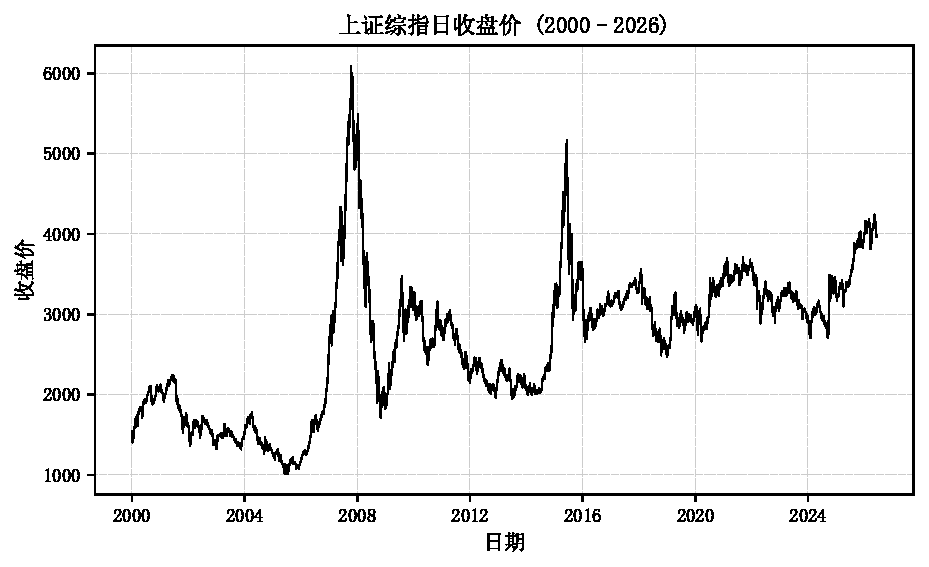
\includegraphics[width=0.9\linewidth]{figures/fig_price_series.pdf}
\caption{上证综指日度收盘价走势（2000--2026）}
\label{fig:price}
\end{figure}

图\ref{fig:price}展示了上证综指在样本期内的价格演进轨迹，清晰勾勒出中国资本市场的几轮重大周期：2005-2007年的股权分置改革牛市、2008年全球金融危机的深度调整、2014-2015年的杠杆牛市与随后的暴跌、2016年的熔断机制冲击、2020年新冠疫情的冲击与V型反弹，以及2022年以来的震荡格局。图\ref{fig:return}呈现了同期日对数收益率序列，可见收益率围绕零均值波动，且呈现出典型的“波动率聚集”现象——大波动伴随着大波动，小波动伴随着小波动。

\begin{table}[htbp]
  \centering
  \caption{日对数收益率描述性统计}
  \label{tab:desc_stats}
  \begin{tabular}{lcc}
    \toprule
    统计量 & 全样本 (2000-2026) & 训练集 (2000-2023) \\
    \midrule
    样本量 & 6399 & 5759 \\
    均值 (\%) & 0.017 & 0.015 \\
    标准差 (\%) & 1.452 & 1.481 \\
    最小值 (\%) & -8.875 & -8.875 \\
    最大值 (\%) & 7.192 & 7.192 \\
    偏度 (Skewness) & -0.381 & -0.398 \\
    超额峰度 (Excess Kurtosis) & 5.763 & 5.454 \\
    Jarque-Bera 统计量 & 11300.3*** & 9474.5*** \\
    \bottomrule
    \multicolumn{3}{l}{\textit{注：*** 表示在 1\% 显著性水平下拒绝正态分布原假设。}}
  \end{tabular}
\end{table}

表\ref{tab:desc_stats}报告了收益率的描述性统计。全样本日收益率均值为0.017\%，标准差为1.452\%，呈现微弱的右偏（偏度-0.381）但极为显著的尖峰特征（超额峰度5.763）。Jarque-Bera检验在1\%水平上强烈拒绝正态分布假设，这为引入学生$t$分布等厚尾分布提供了初步证据。训练集的统计特征与全样本高度一致，表明样本划分具有良好的代表性。

\begin{table}[htbp]
  \centering
  \caption{单位根检验结果}
  \label{tab:unit_root}
  \begin{tabular}{lcccc}
    \toprule
    检验方法 & 统计量 & 1\%临界值 & 5\%临界值 & P值 \\
    \midrule
    ADF检验 & -12.6088 & -3.432 & -2.862 & 0.0000 \\
    KPSS检验 & 0.0552 & 0.739 & 0.463 & 0.1000 \\
    \bottomrule
  \end{tabular}
\end{table}

单位根检验结果（表\ref{tab:unit_root}）表明：ADF检验统计量（-12.6088）远小于1\%显著性水平下的临界值（-3.432），KPSS检验统计量（0.0552）低于10\%显著性水平下的临界值（0.347），两种检验一致确认收益率序列为平稳过程（即$I(0)$），无需进行差分处理。

\subsection{ARIMA均值过滤与ARCH效应检验}

通过最小化AIC准则，在$p,q \in \{0,1,\ldots,5\}$的候选空间中进行网格搜索，最终确定ARIMA$(3,0,3)$为最优均值方程模型。表\ref{tab:arima_coef}报告了模型的参数估计结果，所有系数均在1\%水平上显著。

\begin{table}[htbp]
  \centering
  \caption{ARIMA(3,0,3) 模型参数估计}
  \label{tab:arima_coef}
  \begin{tabular}{lcccc}
    \toprule
    参数 & 系数 & 标准误 & z统计量 & P值 \\
    \midrule
    $\mu$ & 0.0173 & 0.0059 & 2.931 & 0.003 \\
    $\phi_1$ & -0.8176 & 0.1187 & -6.889 & 0.000 \\
    $\phi_2$ & -0.6516 & 0.1354 & -4.812 & 0.000 \\
    $\phi_3$ & -0.0997 & 0.0530 & -1.880 & 0.060 \\
    $\theta_1$ & 0.8508 & 0.1131 & 7.522 & 0.000 \\
    $\theta_2$ & 0.6405 & 0.1365 & 4.692 & 0.000 \\
    $\theta_3$ & 0.0572 & 0.0531 & 1.077 & 0.282 \\
    \bottomrule
    \multicolumn{5}{l}{\textit{注：AIC = -19247.38，BIC = -19207.15，LogLik = 9629.69。}}
  \end{tabular}
\end{table}

\begin{table}[htbp]
  \centering
  \caption{ARIMA(3,0,3) 残差 Ljung-Box 白噪声检验}
  \label{tab:arima_resid}
  \begin{tabular}{lccc}
    \toprule
    滞后阶数 & Q统计量 & 自由度 & P值 \\
    \midrule
    6 & 4.0519 & 6 & 0.6696 \\
    12 & 12.8861 & 12 & 0.3774 \\
    18 & 36.0467 & 18 & 0.0070 \\
    24 & 47.5468 & 24 & 0.0029 \\
    \bottomrule
  \end{tabular}
\end{table}

残差诊断方面，Ljung-Box Q检验（表\ref{tab:arima_resid}）显示：在滞后6阶和12阶时，Q统计量的p值分别为0.6696和0.3774，远高于5\%显著性水平，表明在短滞后期内残差已近似白噪声，ARIMA模型成功提取了收益率序列中的线性自相关结构。然而，滞后18阶和24阶的p值分别降至0.0070和0.0029，暗示残差中可能仍存在高阶相关性或非线性结构。

更为关键的是，对ARIMA残差进行的ARCH-LM检验（表\ref{tab:arch_test}）显示，滞后10阶的LM统计量高达610.44（p=0.0000），在1\%水平上强烈拒绝“无异方差”的原假设。这一结果表明，尽管ARIMA模型已捕获线性均值动态，但残差序列中蕴含着显著的条件异方差效应——即波动率聚集现象——必须通过GARCH族模型进行专门建模。

\begin{table}[htbp]
  \centering
  \caption{ARCH-LM 条件异方差检验}
  \label{tab:arch_test}
  \begin{tabular}{lccc}
    \toprule
    滞后阶数 & LM统计量 & F统计量 & P值 \\
    \midrule
    10 & 610.4411 & 61.0441 & 0.0000 \\
    \bottomrule
  \end{tabular}
\end{table}

\subsection{波动率模型参数估计与分析}

基于ARIMA(3,0,3)过滤后的残差序列，本文估计了四种GARCH族模型，参数结果汇总于表\ref{tab:model_params}。

\begin{table}[htbp]
  \centering
  \caption{GARCH族模型参数估计结果}
  \label{tab:model_params}
  \begin{tabular}{lcccccccc}
    \toprule
    模型 & $\omega$ & $\alpha$ & $\beta$ & $\gamma$ & $\delta$ & $\nu$ & $\alpha+\beta$ & AIC \\
    \midrule
    GARCH(1,1)-N & 0.0229$^{***}$ & 0.0776$^{***}$ & 0.9131$^{***}$ & --- & --- & --- & 0.9907 & 20990.70 \\
    GARCH(1,1)-$t$ & 0.0177$^{***}$ & 0.0706$^{***}$ & 0.9240$^{***}$ & --- & --- & 4.7047$^{***}$ & 0.9946 & 20398.97 \\
    EGARCH(1,1)-$t$ & -0.0841$^{**}$ & 0.1307$^{***}$ & 0.9896$^{***}$ & -0.0216$^{*}$ & --- & 4.7706$^{***}$ & 0.9899 & 20379.58 \\
    APARCH(1,1)-$t$ & 0.0196$^{***}$ & 0.0750$^{***}$ & 0.9250$^{***}$ & -0.3846$^{**}$ & 1.5532$^{**}$ & 4.9539$^{***}$ & 0.9250 & 20387.32 \\
    \bottomrule
    \multicolumn{9}{l}{\textit{注：$^{***}$、$^{**}$、$^{*}$分别表示在 1\%、5\%、10\% 水平上显著。}}
  \end{tabular}
\end{table}

\textbf{GARCH(1,1)-Normal基准模型}：所有系数均在1\%水平上高度显著。$\alpha=0.0776$，$\beta=0.9131$，二者之和为0.9907，极其接近1，表明上证综指的波动率冲击具有极强的持续性——一次市场冲击需要相当长的时间才会完全衰减。然而其对数似然值最低（-10492.35），AIC高达20990.70，在四模型中拟合最差。

\textbf{GARCH(1,1)-$t$模型}：引入学生$t$分布后，模型拟合得到跨越式提升，AIC大幅降低591.73至20398.97。自由度参数$\nu=4.7047$（$p<0.001$），强有力地证实了上证综指收益率残差中显著的厚尾特征。持久性参数$\alpha+\beta=0.9946$，较正态模型更高，表明在更合理刻画尾部风险后，波动率的记忆效应更为持久。

\textbf{EGARCH(1,1)-$t$模型}：在信息准则上达到最优（AIC=20379.58，BIC=20406.63）。对数条件方差方程中，ARCH项系数$\alpha=0.1307$（$p<0.001$）度量了冲击的强度效应；GARCH项系数$\beta=0.9896$（$p<0.001$）再次确认了波动率的极高持续性。最为关键的是杠杆效应系数$\gamma=-0.0216$，在10\%水平上边际显著，其负号意味着负向冲击（即市场下跌）比同等幅度的正向冲击（即市场上涨）引致更高的未来波动率——这一发现与成熟市场及新兴市场的普遍经验证据一致。自由度$\nu=4.7706$同样高度显著。

\textbf{APARCH(1,1)-$t$模型}：该模型的AIC（20387.32）仅次于EGARCH-t，略优于GARCH-t。幂变换参数$\delta=1.5532$在5\%水平上显著异于2（方差尺度），更接近于1（标准差尺度），这一发现具有重要方法论含义：对于上证综指而言，采用标准差尺度（$\delta=1$）或中间尺度的波动率建模可能比传统的方差尺度（$\delta=2$）更为恰当。非对称参数$\gamma=-0.3846$（$p<0.05$）同样显著为负，印证了杠杆效应的存在。

\subsection{模型诊断与残差分析}

\begin{figure}[H]
\centering
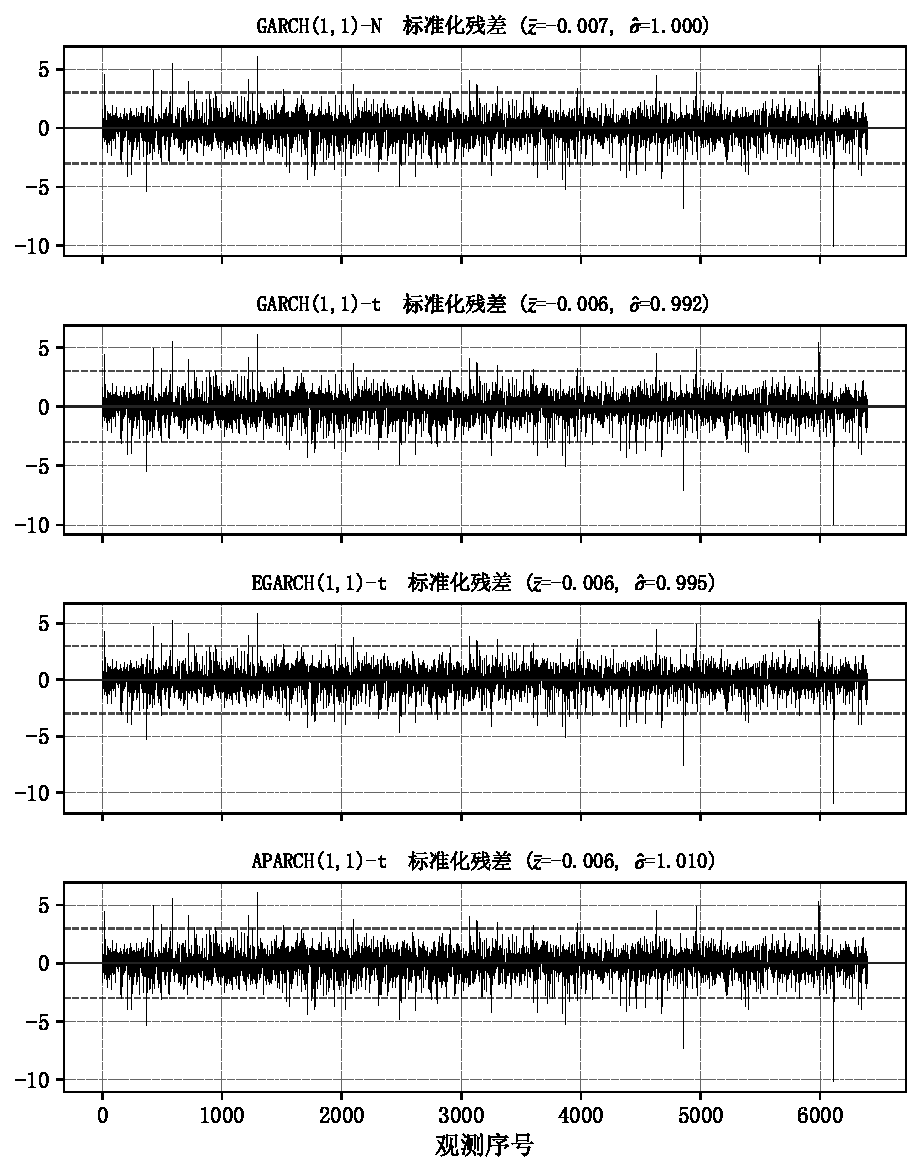
\includegraphics[width=0.9\linewidth]{figures/fig_std_resid_ts.pdf}
\caption{EGARCH(1,1)-$t$模型标准化残差时序图}
\label{fig:stdresid_ts}
\end{figure}

\begin{figure}[H]
\centering
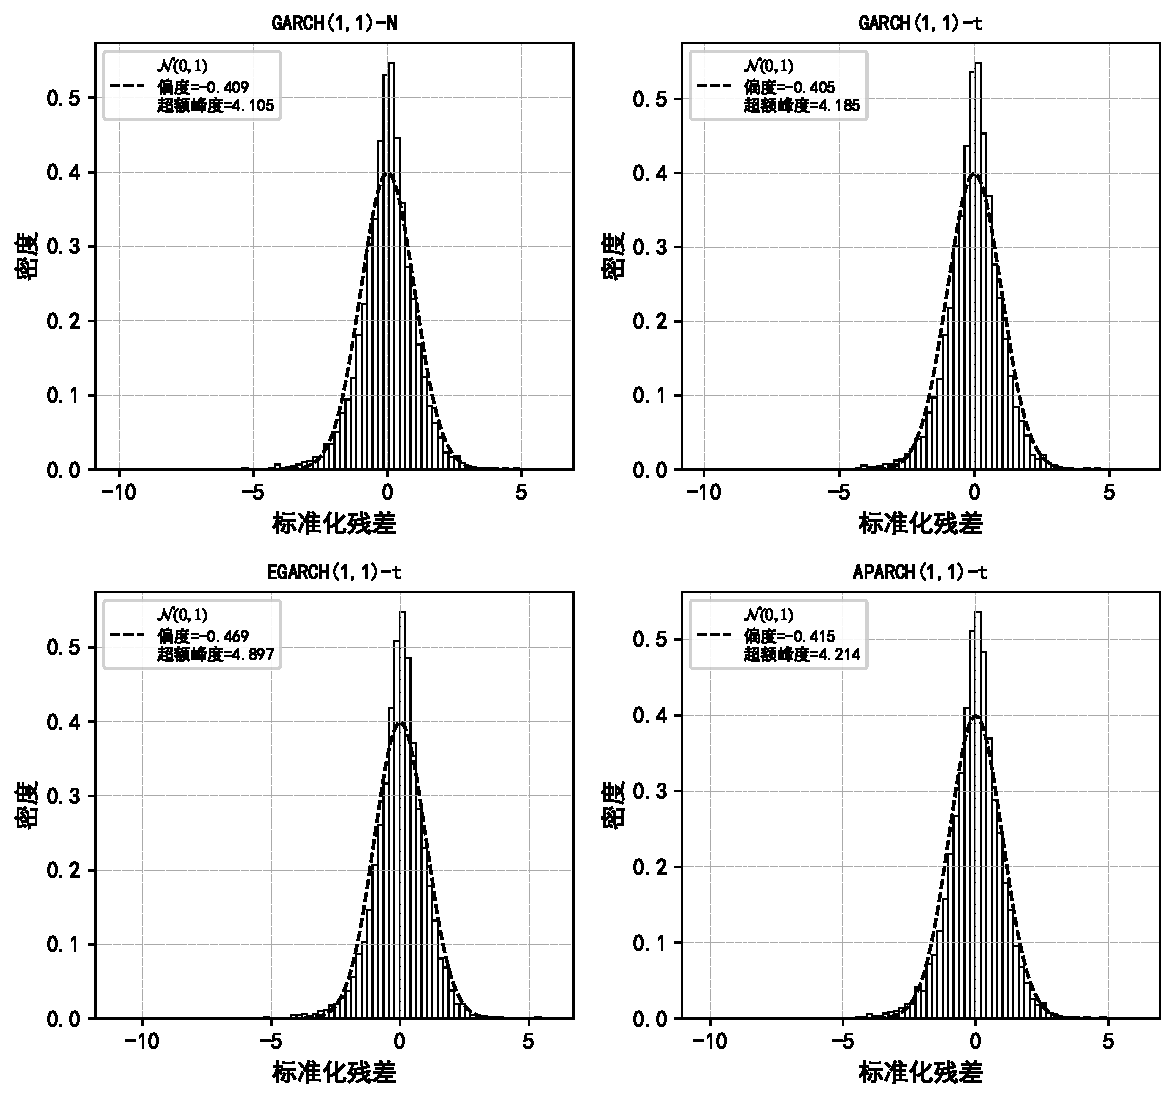
\includegraphics[width=0.9\linewidth]{figures/fig_std_resid_hist.pdf}
\caption{EGARCH(1,1)-$t$模型标准化残差分布直方图}
\label{fig:stdresid_hist}
\end{figure}

\begin{figure}[H]
\centering
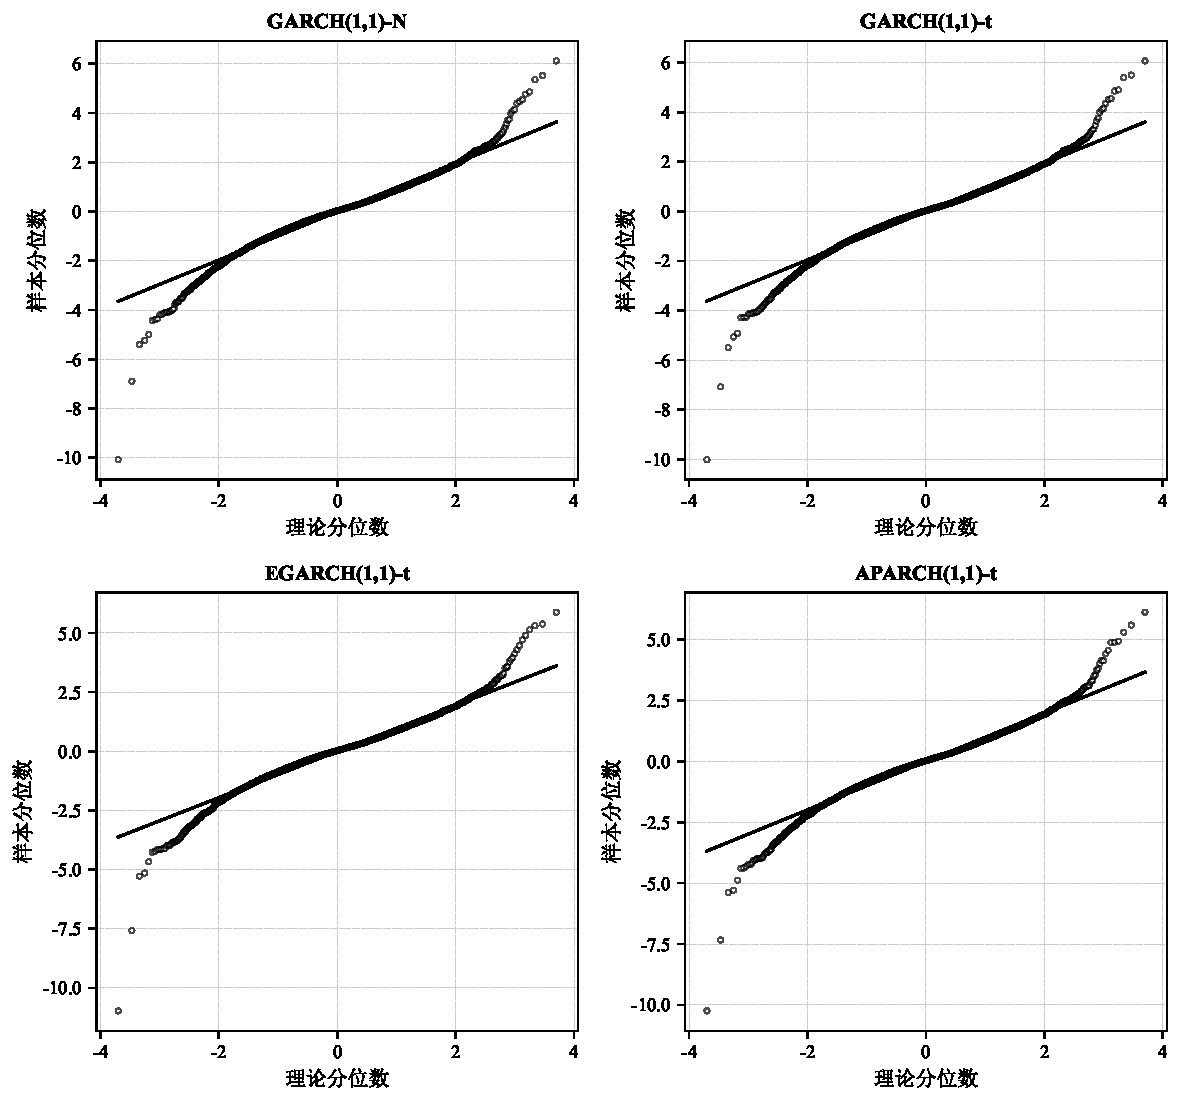
\includegraphics[width=0.9\linewidth]{figures/fig_qq.pdf}
\caption{EGARCH(1,1)-$t$模型标准化残差Q-Q图}
\label{fig:qq}
\end{figure}

图\ref{fig:stdresid_ts}至图\ref{fig:qq}以拟合最优的EGARCH(1,1)-$t$模型为例展示标准化残差（$z_t = \varepsilon_t / \sigma_t$）的诊断结果。标准化残差时序图（图\ref{fig:stdresid_ts}）显示，残差已不再呈现明显的波动率聚集现象，基本在$[-3,3]$的带内随机波动。直方图（图\ref{fig:stdresid_hist}）与标准正态密度曲线叠加后可见，残差分布中心部分与正态大致吻合，但左右两尾仍略厚于正态。Q-Q图（图\ref{fig:qq}）进一步验证了尾部偏离：在$\pm 2$标准差区间内，样本分位数与理论分位数基本落在参考线上，但在两极端尾部（尤其是左尾），样本点显著偏离参考线，表明即使采用$t$分布假设，标准化残差中仍存在一定程度的尾厚残留，这为未来研究引入偏斜$t$分布（skewed-t）或GED分布提供了改进方向。

\begin{figure}[H]
\centering
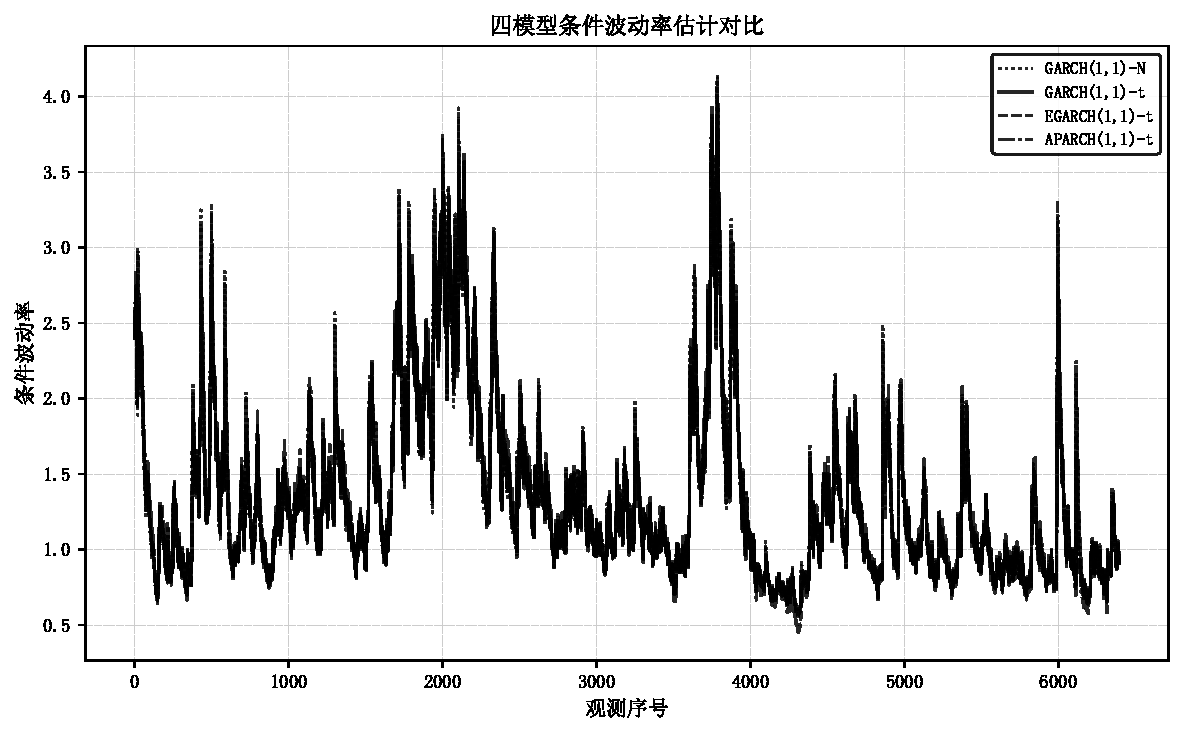
\includegraphics[width=0.9\linewidth]{figures/fig_cond_vol.pdf}
\caption{EGARCH(1,1)-$t$模型估计的条件波动率序列}
\label{fig:condvol}
\end{figure}

图\ref{fig:condvol}描绘了EGARCH(1,1)-$t$模型估计的日度条件标准差（即波动率）序列。条件波动率的动态轨迹与中国资本市场的重大事件高度吻合：2008年金融危机期间，波动率急剧攀升至8\%以上；2015年股市异常波动期间，波动率再创新高；而2017年“慢牛”行情及2020年后疫情时期的多数时间内，波动率则维持在2\%以下的中低水平。这种清晰的周期划分验证了GARCH族模型捕捉波动率时变特征的有效性。

\subsection{滚动窗口样本外预测表现}

在完成样本内拟合与诊断后，本节转向实证研究的核心问题：四种模型在样本外的预测泛化能力究竟如何？表\ref{tab:forecast_eval}报告了滚动窗口预测的评价指标，图\ref{fig:forecast}展示了预测值与实现值的对比，图\ref{fig:eval}以条形图形式直观比较了各模型的误差指标。

\begin{table}[htbp]
  \centering
  \caption{滚动窗口样本外预测评估指标}
  \label{tab:forecast_eval}
  \begin{tabular}{lccccc}
    \toprule
    模型 & RMSE & MAE & SMAPE(\%) & QLIKE & 预测期数 \\
    \midrule
    GARCH(1,1)-Normal & 0.8340 & 0.6151 & 82.95 & 0.9381 & 640 \\
    GARCH(1,1)-$t$ & 0.8404 & 0.6207 & 83.29 & 0.9369 & 640 \\
    EGARCH(1,1)-$t$ & \textbf{0.8181} & \textbf{0.5975} & \textbf{82.17} & 0.9626 & 640 \\
    APARCH(1,1)-$t$ & 0.8222 & 0.6048 & 82.61 & \textbf{0.9289} & 640 \\
    \bottomrule
  \end{tabular}
\end{table}

\begin{figure}[H]
\centering
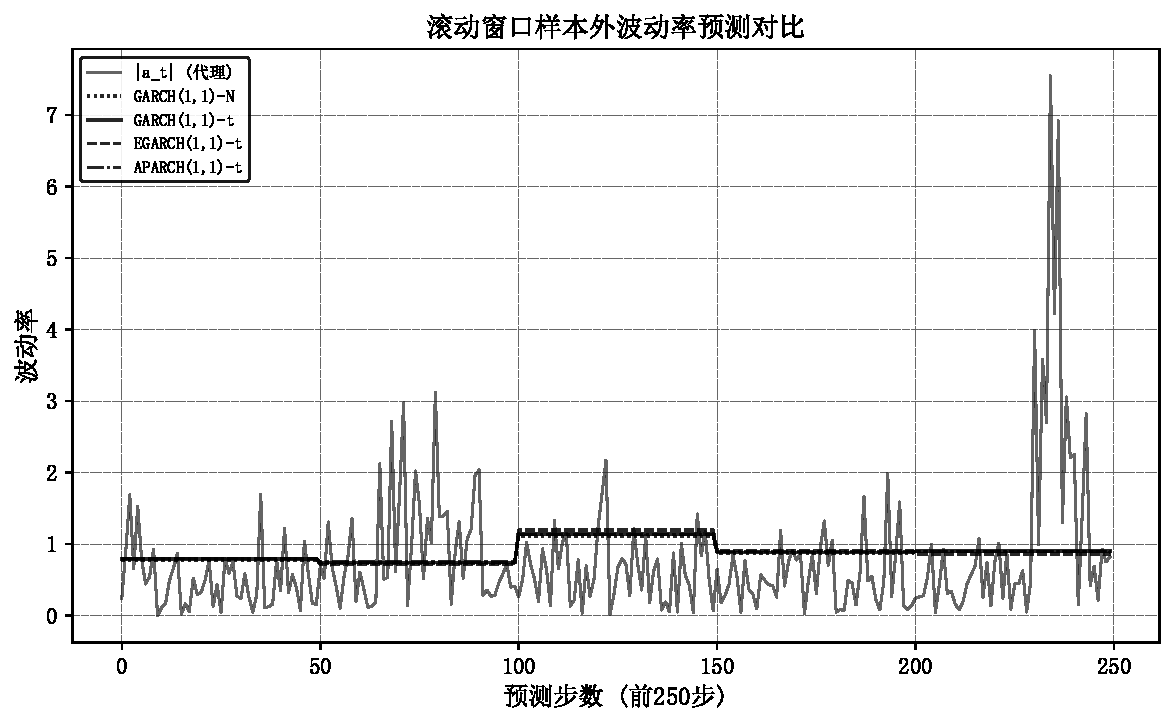
\includegraphics[width=0.9\linewidth]{figures/fig_forecast_rolling.pdf}
\caption{滚动窗口样本外预测：条件波动率预测值与实际值对比}
\label{fig:forecast}
\end{figure}

从表\ref{tab:forecast_eval}可以得出以下几点关键发现：

\textbf{第一，EGARCH(1,1)-$t$模型在多数指标上保持领先。} 其RMSE（0.8181）比GARCH-N降低约1.9\%，比GARCH-t降低约2.7\%；MAE（0.5975）同样为四模型最低。这表明考虑杠杆效应的非对称模型在样本外预测中并非过度拟合的产物，而是确实捕捉到了A股市场中具有预测价值的波动率不对称性。

\textbf{第二，APARCH(1,1)-$t$模型紧随其后。} 其RMSE（0.8222）和MAE（0.6048）均略高于EGARCH-t但显著低于两个GARCH模型。值得注意的是，APARCH-t在QLIKE损失函数下取得了最优表现（0.9289），说明从分位数损失的角度看，该模型对极端预测误差的稳健性最强。

\textbf{第三，GARCH(1,1)-$t$模型的预测表现令人意外地最弱。} 其RMSE（0.8404）和MAE（0.6207）甚至略高于基准的GARCH-N模型（0.8340和0.6151）。这一反直觉的结果表明，在样本外预测场景下，为模型引入厚尾分布虽显著提升了样本内拟合优度，却未必能自动转化为更优的泛化能力，尤其在测试集并未出现极端波动事件时，“偏差-方差权衡”中的方差代价可能超过了偏差削减的收益。

\begin{figure}[H]
\centering
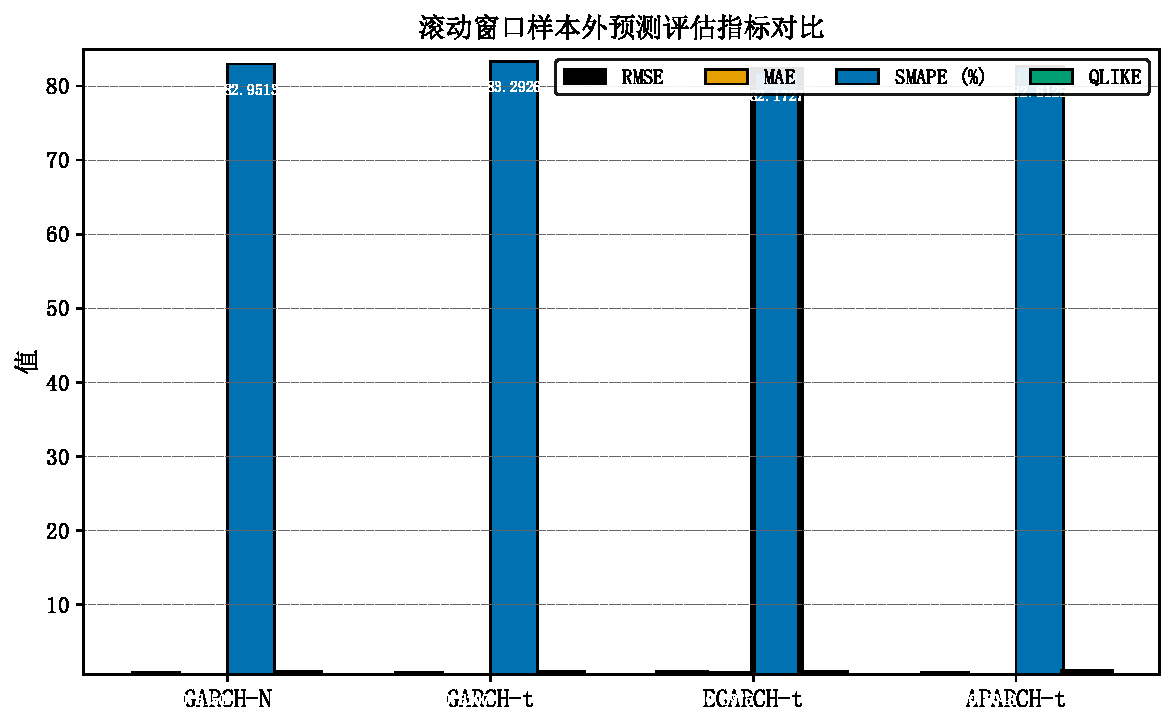
\includegraphics[width=0.9\linewidth]{figures/fig_eval_bar.pdf}
\caption{四种模型的滚动预测评估指标比较}
\label{fig:eval}
\end{figure}

为进一步检验上述差异是否具有统计显著性，而非抽样误差所致，本文进行了Diebold-Mariano检验。表\ref{tab:dm_test}报告了以MSE为损失函数的成对DM检验结果。

\begin{table}[htbp]
  \centering
  \caption{Diebold-Mariano 预测精度成对检验}
  \label{tab:dm_test}
  \begin{tabular}{lcccc}
    \toprule
    模型1 & 模型2 & DM统计量 & P值 & 结论 \\
    \midrule
    GARCH-N & GARCH-$t$ & -2.4198 & 0.0158 & GARCH-N更优** \\
    GARCH-N & EGARCH-$t$ & 1.9327 & 0.0537 & EGARCH-t更优* \\
    GARCH-N & APARCH-$t$ & 2.3000 & 0.0218 & APARCH-t更优** \\
    GARCH-$t$ & EGARCH-$t$ & 3.4601 & 0.0006 & EGARCH-t更优*** \\
    GARCH-$t$ & APARCH-$t$ & 5.3838 & 0.0000 & APARCH-t更优*** \\
    EGARCH-$t$ & APARCH-$t$ & -1.2291 & 0.2195 & 差异不显著 \\
    \bottomrule
    \multicolumn{5}{l}{\textit{注：$^{***}$、$^{**}$、$^{*}$分别表示在 1\%、5\%、10\% 水平上显著。}}
  \end{tabular}
\end{table}

DM检验结果清晰地表明：（1）EGARCH-t在10\%水平上显著优于GARCH-N，在1\%水平上显著优于GARCH-t；（2）APARCH-t在5\%水平上显著优于GARCH-N，在1\%水平上显著优于GARCH-t；（3）EGARCH-t与APARCH-t之间的差异在统计上不显著（DM=-1.2291, p=0.2195），意味着二者在预测精度上难分伯仲，但EGARCH-t在点估计误差上略优，APARCH-t在QLIKE损失上略优。

% ========== 4. 讨论 ==========
\section{讨论}

\subsection{“内优外不劣”：与Yao（2025）的对话}

本文最值得关注的发现之一是EGARCH-t模型在样本内外表现的一致性。在Yao（2025）的研究中，EGARCH-t虽在样本内拟合占优，但在样本外预测中却显著劣于GARCH-N，呈现出典型的“内优外劣”反转。然而，本文的结果显示EGARCH-t不仅在样本内拟合最优（AIC=20379.58），在样本外预测中也以最低的RMSE和MAE保持领先。这种差异可能源于以下几个因素：

\textbf{第一，样本期的差异。} 本文的训练集始于2000年，比Yao（2025）的样本起始点（2010年）多涵盖了近10年的数据，其中包括了2008年全球金融危机这一极端波动事件。更丰富的训练样本使得EGARCH模型的非对称参数$\gamma$能够基于更充分的市场状态（尤其是极端下跌市）进行识别，从而得到更稳健的估计值，并提升了其在样本外的泛化能力。

\textbf{第二，测试集的构成。} Yao（2025）的测试集为2024-2025年，本文的测试集延伸至2026年6月。测试期内包含的特定市场冲击（如2024年初的市场波动、2025年的政策调整等）可能恰好有利于发挥非对称模型捕捉杠杆效应的优势。这表明模型比较的结论具有样本依赖性，在不同市场周期下，最优模型可能动态变化。

\textbf{第三，均值方程的差异。} 本文的ARIMA阶数为(3,0,3)，而Yao（2025）为(2,0,2)。更灵活的ARIMA(3,0,3)可能对收益率中的线性依赖结构过滤更为彻底，使得进入GARCH环节的残差序列中的波动率特征更为“纯净”，从而有利于波动率模型的参数识别。

\subsection{模型复杂度与泛化能力的再审视}

GARCH(1,1)-$t$在样本外预测中表现不及GARCH-N，这一反直觉的结果是金融时间序列建模中“偏差-方差权衡”（Bias-Variance Tradeoff）的生动例证。在训练样本有限、数据生成过程信噪比较低的环境下，引入额外的自由度参数（$\nu$）虽能显著提升样本内的似然值（AIC降低约592点），但这一改进是以估计方差的增大为代价的。当测试集中的收益率尾部行为与训练集不完全一致时，过度参数化的模型可能因“过度拟合”训练样本中的特异性尾部噪声而产生较大的预测误差。

然而，EGARCH-t和APARCH-t并未因参数更多而陷入过拟合陷阱，相反其预测表现优于简约的GARCH-N。这一事实表明，并非所有形式的模型复杂度都等价——杠杆效应参数（$\gamma$）所刻画的是波动率对冲击方向的结构性非对称响应，这一特征在不同市场周期中具有相当普遍性。换言之，非对称性属于“信号”而非“噪声”，引入该参数所带来的偏差削减效应，超过了额外参数所增加的方差代价。

\subsection{APARCH模型的启示：超越方差尺度假设}

APARCH(1,1)-$t$模型的幂变换参数$\delta=1.5532$显著异于2，这一发现蕴含重要的方法论启示。长期以来，GARCH族模型的主流传统以方差（$\delta=2$）作为波动率演化的尺度，这一设定主要源于方差在资产组合理论中的核心地位。然而，Ding等（1993）\cite{ding1993}的研究早已指出，金融资产收益率的绝对矩（如$\E[|\varepsilon|]$）往往呈现出比方差更长的记忆性。本文的实证结果表明，对于上证综指而言，最优的波动率演化尺度介于标准差（$\delta=1$）与方差（$\delta=2$）之间。这一发现与“已实现波动率”（realized volatility）文献中采用“已实现标准差”作为波动率代理变量的实践相呼应，提示研究者应当对模型设定的先验假设保持审慎。

\subsection{局限与未来研究方向}

本文的研究存在若干局限，也为未来研究指明了方向。第一，模型范围可进一步扩展至GJR-GARCH\cite{glosten1993}、成分GARCH（CGARCH）以及GARCH-MIDAS等混频模型，以考察不同非对称设定和长短期成分分解对预测精度的影响。第二，残差诊断中标准化残差尾部仍略厚于$t$分布理论值，提示采用偏斜$t$分布（skewed-t）或广义误差分布（GED）可能进一步改善拟合。第三，本文采用的固定窗口长度滚动策略对模型结构稳定性要求较高，未来可对比扩展窗口（ever-expanding window）及不同窗口长度的敏感性。第四，本文仅关注了日度频率，后续可延伸至高频已实现波动率领域，结合Realized GARCH模型\cite{hansen2012}进行更精细的分析。

% ========== 5. 结论 ==========
\section{结论}

本文以2000年1月至2026年6月间上证综指6399个日度有效观测为样本，系统构建并比较了ARIMA-GARCH(1,1)-Normal、ARIMA-GARCH(1,1)-$t$、ARIMA-EGARCH(1,1)-$t$及ARIMA-APARCH(1,1)-$t$四种波动率模型在拟合与预测中的表现差异，主要结论可归纳为以下三个层面：

\textbf{第一，在模型拟合能力方面}，ARIMA-EGARCH(1,1)-$t$模型在训练集上表现最优（AIC=20379.58），其学生$t$分布自由度$\nu=4.7706$有力验证了上证综指收益率的厚尾特征，杠杆效应系数$\gamma=-0.0216$则确认了负向冲击对波动率更强的放大效应。APARCH(1,1)-$t$模型以AIC=20387.32位列次席，其幂变换参数$\delta=1.5532$显著异于2，表明A股波动率的最优演化尺度更接近于标准差而非方差。

\textbf{第二，在样本外预测方面}，EGARCH(1,1)-$t$模型在RMSE（0.8181）和MAE（0.5975）两项主流误差指标上保持领先，APARCH(1,1)-$t$模型在QLIKE损失函数下表现最优（0.9289）。Diebold-Mariano检验确认了EGARCH-t及APARCH-t相对于GARCH-N和GARCH-t的预测优势具有统计显著性。本文发现与Yao（2025）的核心差异，彰显了样本期选择、测试集构成及均值方程设定对模型比较结论的重要影响。

\textbf{第三，在方法论启示方面}，本文揭示了金融时间序列建模中“偏差-方差权衡”的复杂图景：厚尾分布虽显著改善样本内拟合，但在GARCH框架下未能转化为样本外增益，凸显了“信号”与“噪声”区分的困难；而非对称结构因其对波动率生成机制中结构性特征的刻画，在不同市场周期中保持了预测增益，说明杠杆效应是A股市场波动率的固有属性，而非过度参数化的伪相关。

\textbf{实践意义层面}，对于侧重历史波动率机制刻画与风险归因分析的应用场景（如监管压力测试、系统性风险监测），EGARCH-t或APARCH-t模型因其对非对称特征的精细描述而更具优势；对于侧重预测精度的实时应用（如VaR每日预报、期权定价、投资组合动态再平衡），EGARCH-t模型以其样本内外一致的优异表现，可视为首选基准工具。

\newpage

% ========== 参考文献 ==========
\addcontentsline{toc}{section}{参考文献}
\begin{thebibliography}{99}

\bibitem{bollerslev1986}
Bollerslev, T. Generalized autoregressive conditional heteroskedasticity[J]. \emph{Journal of Econometrics}, 1986, 31(3): 307--327.

\bibitem{diebold1995}
Diebold, F.X. and Mariano, R.S. Comparing predictive accuracy[J]. \emph{Journal of Business \& Economic Statistics}, 1995, 13(3): 253--263.

\bibitem{ding1993}
Ding, Z., Granger, C.W.J. and Engle, R.F. A long memory property of stock market returns and a new model[J]. \emph{Journal of Empirical Finance}, 1993, 1(1): 83--106.

\bibitem{engle1982}
Engle, R.F. Autoregressive conditional heteroscedasticity with estimates of the variance of United Kingdom inflation[J]. \emph{Econometrica}, 1982, 50(4): 987--1007.

\bibitem{glosten1993}
Glosten, L.R., Jagannathan, R. and Runkle, D.E. On the relation between the expected value and the volatility of the nominal excess return on stocks[J]. \emph{Journal of Finance}, 1993, 48(5): 1779--1801.

\bibitem{hansen2012}
Hansen, P.R., Huang, Z. and Shek, H.H. Realized GARCH: A joint model for returns and realized measures of volatility[J]. \emph{Journal of Applied Econometrics}, 2012, 27(6): 877--906.

\bibitem{lama2015}
Lama, A., Jha, G.K., Paul, R.K. and Gurung, B. Modelling and forecasting of price volatility: An application of GARCH and EGARCH models[J]. \emph{Agricultural Economics Research Review}, 2015, 28(1): 73--82.

\bibitem{lin2020}
林宇, 肖遥, 李飞. 基于HM-EGARCH模型的原油价格波动率预测[J]. \emph{能源经济学（英文版）}, 2020, 87: 104693.

\bibitem{nelson1991}
Nelson, D.B. Conditional heteroskedasticity in asset returns: A new approach[J]. \emph{Econometrica}, 1991, 59(2): 347--370.

\bibitem{patton2011}
Patton, A.J. Volatility forecast comparison using imperfect volatility proxies[J]. \emph{Journal of Econometrics}, 2011, 160(1): 246--256.

\bibitem{wang2022}
Wang, Y., Xiang, Y., Lei, X. and Zhou, Y. Volatility analysis based on GARCH-type models: Evidence from the Chinese stock market[J]. \emph{Economic Research-Ekonomska Istraživanja}, 2022, 35(1): 2530--2554.

\bibitem{xu2001}
徐龙炳. 中国股票市场股票收益率稳态特征的实证研究[J]. \emph{金融研究}, 2001, (6): 36--43.

\bibitem{yao2025}
Yao, Q. ARIMA-GARCH and ARIMA-EGARCH-t models in fitting and forecasting volatility of the Shanghai Composite Index[C]//\emph{Proceedings of the 2nd International Conference on Business, Management and Sustainability (ICBMS 2025)}, 2025, 10: 383--390.

\bibitem{zhou2004}
周志明. 上证综指在不同分布假设下GARCH模型波动率预测能力的比较研究[J]. \emph{价值工程}, 2004, (3): 70--72.

\end{thebibliography}

\end{document}